\chapter{Resultados y Análisis de Impacto}

\section{Resultados}

\subsection{Costes computacionales}
El entrenamiento del modelo ocupó en torno a los 4GB de RAM y  10GB de VRAM. 
El tiempo de ocupación de la gpu era en torno al 20\% del total, permitiendo el uso del ordenador para otras tareas como la redacción de esta memoria durante el transcurso del entrenamiento.
\subsection{Evaluación del modelo}
Según expuesto por Ebony Mayhorn en el reporte de 2023 del Multidisciplinary Digital Publishing Institute.  Actualmente, no existe ningún estándar que permita realizar comparativas entre diferentes tecnologías NILM \autocite{NILMreview2023} \autocite{mayhorn2015load}

Para evaluar el modelo, se hace uso de métricas definidas por Ang Gao en \autocite{GAO2023109443}: accuracy, F1 score, y weighted F1 score\footnote{modificadas para el análisis multi-etiqueta}.
Por ello, y por el enfoque del proyecto, no se exponen comparaciones entre otros modelos
\begin{figure}[H]
    \centering
    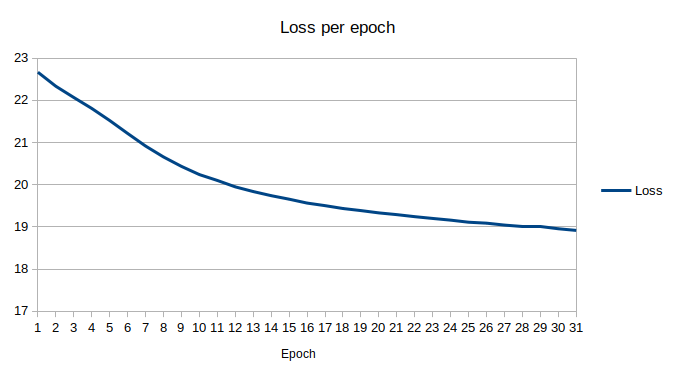
\includegraphics[height=150px]{images/Losstable.png}
    \caption{Pérdida total del modelo durante el entrenamiento}
    \label{fig:loss}
\end{figure}

Como podemos observar en \ref{fig:loss} la pérdida disminuye consistentemente a lo largo del entrenamiento. Una pérdida decreciente típicamente significa que el modelo está aprendiendo y minimizando el error con el tiempo.

\begin{figure}[htbp]
    \centering
    \begin{minipage}[b]{0.495\textwidth}
        \centering
        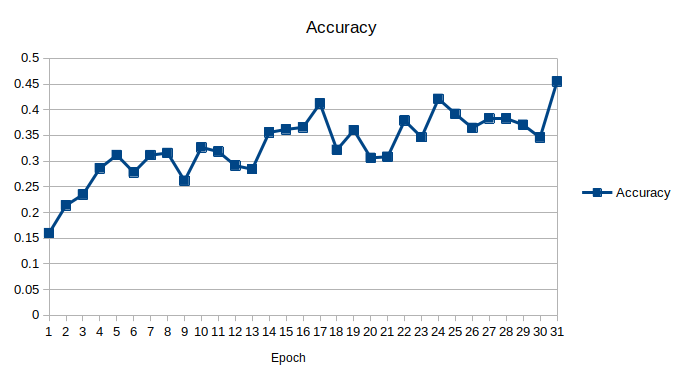
\includegraphics[width=\textwidth]{images/Accuracytable.png}
        \caption{Precisión del modelo}
        \label{fig:accuracy}
    \end{minipage}
    \hfill
    \begin{minipage}[b]{0.495\textwidth}
        \centering
        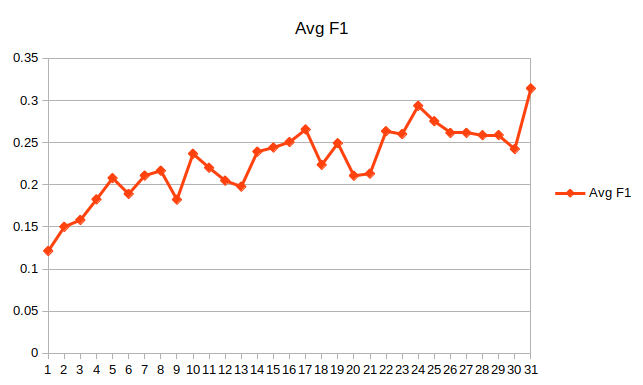
\includegraphics[width=\textwidth]{images/Avgf1table.png}
        \caption{Puntuaje F1 Promedio}
        \label{fig:avgf1}
    \end{minipage}
    \vfill
    \begin{minipage}[b]{0.495\textwidth}
        \centering
        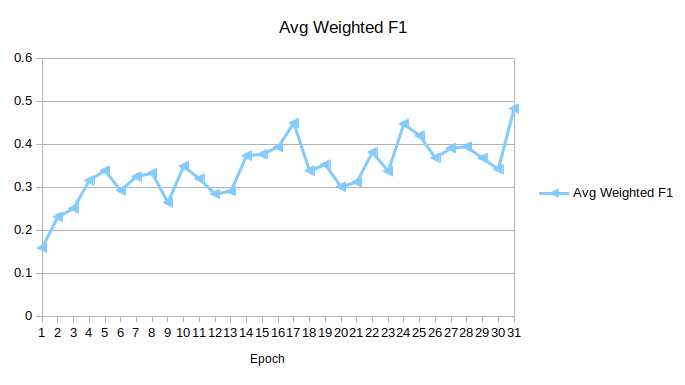
\includegraphics[width=\textwidth]{images/Avgweightedf1table.png}
        \caption{Puntaje F1 Ponderado Promedio}
        \label{fig:avgweightedf1}
    \end{minipage}
    \hfill
    \begin{minipage}[b]{0.495\textwidth}
        \centering
        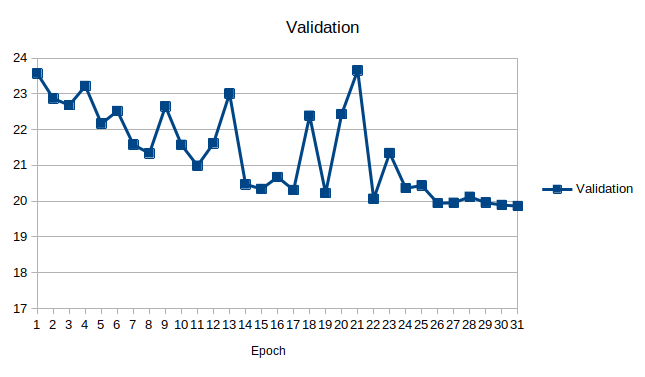
\includegraphics[width=\textwidth]{images/Validationtable.png}
        \caption{Validación}
        \label{fig:validation}
    \end{minipage}
    \caption{Métricas del modelo}
    \label{fig:grid}
\end{figure}


Todas las métricas sugieren una mejora general en el rendimiento a lo largo de las épocas. Las métricas de exactitud, puntaje F1 promedio y puntaje F1 ponderado promedio presentan un incremento constante, indicando una mejor capacidad del modelo para clasificar correctamente y manejar el desequilibrio de clases. Sin embargo, se observan fluctuaciones significativas en la pérdida de validación, lo que sugiere la presencia de sobreajuste. Esto se refleja también en los picos observados en la pérdida de validación, que indican que el modelo tiene dificultades para generalizar en algunos puntos del entrenamiento.Las métricas de exactitud, puntaje F1 promedio y puntaje F1 ponderado promedio presentan un incremento constante, indicando una mejor capacidad del modelo para clasificar correctamente y manejar el desequilibrio de clases. Sin embargo, se observan fluctuaciones significativas en la pérdida de validación, lo que sugiere la presencia de sobreajuste. Esto se refleja también en los picos observados en la pérdida de validación, que indican que el modelo tiene dificultades para generalizar en algunos puntos del entrenamiento.

El sobreajuste ocurre cuando un modelo se adapta demasiado bien a los datos de entrenamiento, incluyendo el ruido y los detalles específicos de esos datos, lo que resulta en un rendimiento pobre en datos no vistos. Para prevenir el sobreajuste, se utilizan técnicas como la validación cruzada, la regularización, y la parada temprana. Técnicas que en este trabajo no dieron tiempo a implementarse.

\section{Impacto}
\subsection{Personal}
Ha sido una experiencia académicamente enriquecedora. Ya que cuando se empezó este trabajo, no se tenía prácticamente ningún conocimiento sobre la inteligencia artificial a un nivel que personalmente se considerase razonable. Se termina este trabajo habiendo disfrutado de profundizar en el área de la inteligencia artificial, más allá de lo estrictamente necesario para el desarrollo de este trabajo. 
\subsection{Social}
%%\todo[inline]{Mayor control de gasto, menos privacidad. Analisis de patrones de gastos y por tanto hábitos personaless/de la vivienda}
Dados los resultados del modelo, el impacto de construir un sistema haciendo uso del modelo entrenado tendrían alguna serie de problemas con la detección de clases de dispositivos. Pero obviando esto; o clasificando manualmente los dispositivos presentes dentro de la vivienda. Podría tener un uso muy ventajoso de cara a un usuario. 
A cambio, podría presentar una serie de problemas de privacidad, si no se manejara de forma segura la seguridad del sistema \autocite{osti_2229911}.
\subsection{Empresarial}
%%\todo[inline]{industria: mayor control y más barato. (explicar pq) del gasto energético}
Según Michael C. et. al. 2016 \autocite{osti_1373019}, la implementación de sistemas de monitorización de carga eléctrica no intrusiva en la industria podría tener un impacto positivo en el control de gasto energético, mejora de la eficiencia energética, ahorros energéticos para consumidores y una transición hacia el Internet de las Cosas. osti_1373019
\subsection{Medioambiental}
%%\todo[inline]{pro: aprovechar el consumo/optimizar los patrones de gasto teniendo mayor granularidad y un modelo inferente como el que se ha desarrollado permite construir en un futuro herramientas predictivas de gastos que por tanto pueden aportar info valiosa para modelos más generales (usando estos y otros datos como los metereológicos, mercantiles, mercados, etc) para estimar la demanda esperada y el volumen de energía a generar.}
El potencial de un modelo como este puede beneficiar la implementación de sistemas de optimización de generación y consumo de energía, que podría potenciar el establecimiento de más comunidades solares en España. Además, establecer este tipo de sistemas da pie a la posibilidad de minar datos para poder entrenar modelos más generales que incorporen los datos de consumo de usuarios y otros, como datos metereológicos, precio de la electricidad, etc. Para poder así estimar y gestionar la oferta y demanda. 

Se recomienda analizar también el potencial impacto respecto a los Objetivos de Desarrollo Sostenible (ODS), de la Agenda 2030, que sean relevantes para el trabajo realizado (\href{https://www.un.org/sustainabledevelopment/es/objetivos-de-desarrollo-sostenible/}{ver enlace})
